\section{Einleitung}
\subsection{Erstes Unterkapitel}
Dies ist ein Zitat:
\lipsum[1-2]
Zwar nicht aus diesem Buch, aber hier eine Zitierung. \citep[vgl. ][S. 5-6]{bernstein97}
\subsection{Zweites Unterkapitel}
Unter Bild \ref{pic:bildname} sieht man eine volle Schönheit.
\begin{figure}[ht]
	\centering
	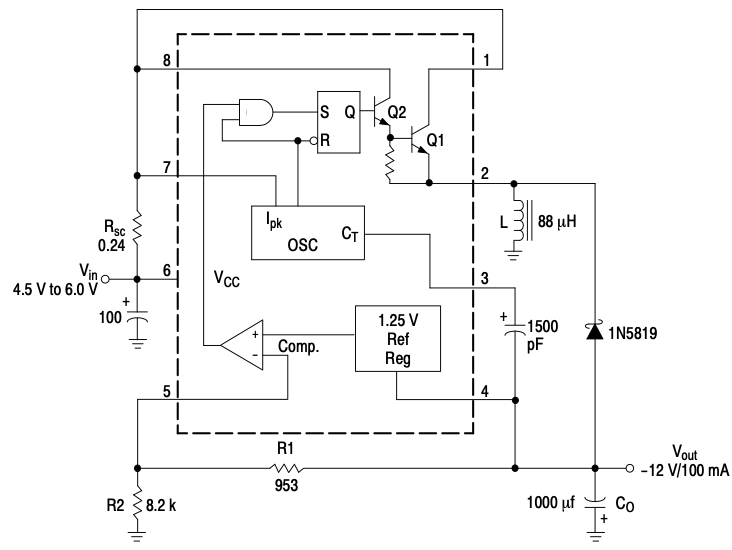
\includegraphics[scale=0.5]{pic/bildname}
	\caption{Beispielbild}
	\label{pic:bildname}
	\quelle \citep[S. 8]{onsemi:MC34063A}
\end{figure}
Ein anderes Bild wird für das Verzeichnis ebenfalls eingefügt.
\begin{figure}[ht]
	\centering
	
\includegraphics[scale=0.5]{pic/title/fhw_logo}
	\caption{Titelbild der FHW}
	\label{pic:titelbild}
\end{figure}

Eine mögliche Abkürzung ist \ac{cad}, sie wird in main.tex definiert. Wenn man dies  ein zweites Mal schreibt, steht nur noch kurz \ac{cad} da. Eine andere Abkürzung wäre \ac{drm}. Möchte man Formelzeichen verwenden, dann deklariert man dieses ebenfalls in main.tex und benutzt dann den dort ausgewählten Befehl. Dieser sollte nur aus Buchstaben bestehen, es darf kein vorhandener Befehl sein. Es ist Empfehlenswert im Befehl m vorweg zu verwenden, um eine mögliche Befehlsüberschneidung auszuschließen. Das Symbol sieht dann so aus: \mEel.

\subsection{Drittes Unterkapitel}
\section{Neuer Abschnitt}
\lipsum[1-3]

Zum Abschluss sollen noch zwei Tabellen dargestellt werden:
\begin{table}[H]
\centering
\begin{tabular}{c c}
Zelle 11 & Zelle 12\\
Zelle 21 & Zelle 22\\
\end{tabular}
\caption{Eine Tabelle}
\label{tab:einetabelle}
\quelle Unbekannt
\end{table}

Die Zweite:
\begin{table}[H]
\centering
\begin{tabular}{l c r}
Zelle 11 & Zelle 12 & Zelle 13\\
Zelle 21 & Zelle 22 & Zelle 23\\
Zelle 31 & Zelle 32 & Zelle 33\\
\end{tabular}
\caption{Eine weitere Tabelle}
\label{tab:eineweiteretabelle}
\end{table}